\chapter{Implementación}

Para la consecución de este proyecto, el desarrollo del software se ha dividido en una serie
de \textbf{hitos}. Un hito, en el desarrollo de software, simboliza un logro, un aspecto
del proyecto que se está cumpliendo conforme se planificó al comienzo del mismo, por tanto, 
éstos son los mejores indicadores del progreso del proyecto para alcanzar los objetivos
finales.\\

A cada hito se le asocia una serie de \textbf{issues} (problemas), los cuáles describen
aspectos a mejorar o solucionar del software durante su desarrollo. \\

Los hitos del proyecto son los siguientes:
\begin{enumerate}
    \item \textbf{\href{https://github.com/alexespana/TFG/milestone/1}{[M1]. Website
    creation}}: creación de la estructura principal de la aplicación web, con las
    principales páginas y funcionalidades. Esta parte será desarrollada en un entorno
    de desarrollo (servidor de desarrollo).
    \item \textbf{\href{https://github.com/alexespana/TFG/milestone/8}{[M2]. Database
    creation}}: creación de las principales tablas para modelar el problema, junto con
    los correspondientes formularios para la recogida de datos en la aplicación web.
    \item \textbf{\href{https://github.com/alexespana/TFG/milestone/2}{[M3]. Authentication}}
    : gestión de usuarios del sitio web, signup, signout, login, logout, cambiar
    contraseña e información de contacto para cada usuario así como third party (social)
    account authentication. 
    \item \textbf{\href{https://github.com/alexespana/TFG/milestone/3}{[M4]. Test behavior}}:
    realización de tests para comprobar el comportamiento de la aplicación.
    \item \textbf{\href{https://github.com/alexespana/TFG/milestone/4}{[M5]. Continuous
    integration}}: el software desarrollado debe integrarse con el posible software
    ya existente en el sitio web, asegurando el correcto funcionaminto de ambos.
    \item \textbf{\href{https://github.com/alexespana/TFG/milestone/5}{[M6]. Log system}}: 
    los eventos más importantes que ocurren en la aplicación deben ser grabados a través
    del uso de un servicio de log. Es conveniente capturar errores en un nivel superior
    de abstracción, evitando modificar código ya hecho.
    \item \textbf{\href{https://github.com/alexespana/TFG/milestone/6}{[M7]. API REST}}:
    el diseño y posterior implementación de la API REST que permita gestionar los recursos
    con los que trabaja la aplicación.
    \item \textbf{\href{https://github.com/alexespana/TFG/milestone/7}{[M8]. Deployment}}:
    el despliegue de la aplicación web en la nube debe realizarse utilizando un dominio
    público y un WSGI (Web Server Gateway Interface).
\end{enumerate}

Si desea tener una vista más general de los milestones, issues, commits, branches, etc del
proyecto puede visitar los siguientes enlaces:

\begin{itemize}
    \item \textbf{\href{https://github.com/alexespana/TFG/milestones}{Milestones}}
    \item \textbf{\href{https://github.com/alexespana/TFG/issues}{Issues}}
    \item \textbf{\href{https://github.com/alexespana/TFG/branches}{Branches}}
    \item \textbf{\href{https://github.com/alexespana/TFG/pulls}{Pull requests}}
\end{itemize}


\section{Website creation}
Para realizar la implementación de las distintas plantillas de la aplicación, se ha hecho
uso del sistema propio de plantillas de Django, llamado \textbf{Django template language},
que es muy parecido a JinJa2 y que está completamente implementado en los backends que
incluye de serie.\\

A la hora de pensar en un diseño para la aplicación web, se ha optado por un diseño
minimalista, que permita diferenciar fácilmente las distintas partes de la aplicación
junto con sus funcionalidades.\\

Es importante mencionar que todas las plantillas del proyecto hacen uso de una plantilla
base que contiene el navegador de la página y el pie de página, por lo que dicha plantilla base
sería tal que así:\\

    \begin{figure}[H]
        \centering
        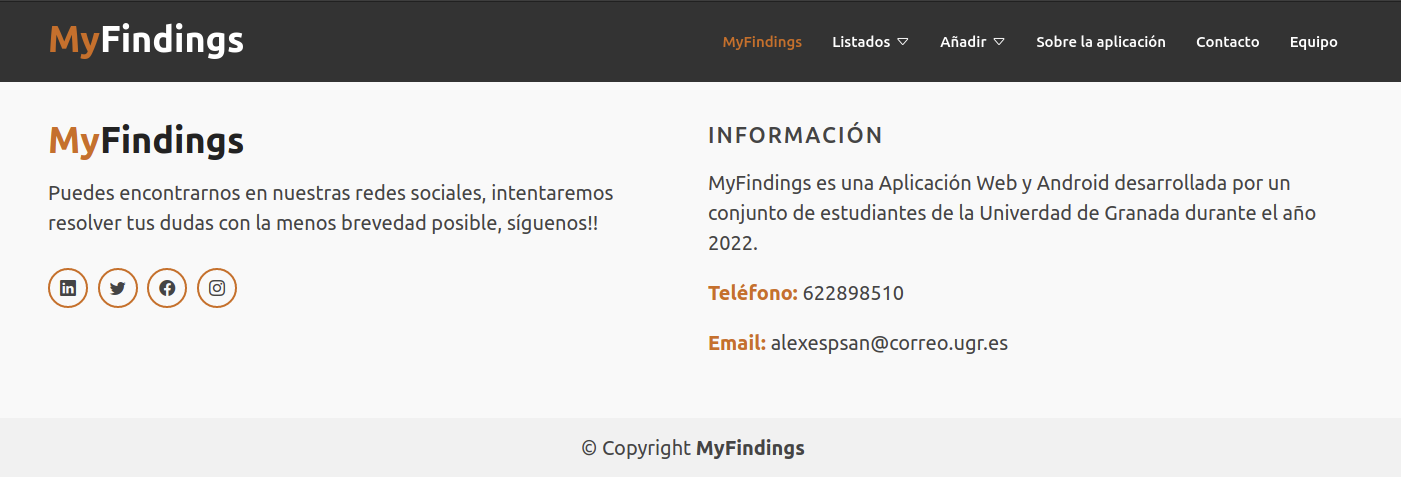
\includegraphics[scale=0.25]{imagenes/base.png}
        \caption{Plantilla base}
        \label{fig:base}
    \end{figure}

El resto de plantillas de este diseño son las que se describen en las secciones siguientes.

    \subsection{Home}
    Ésta es la página principal que se verá al entrar en la aplicación, prácticamente todo el
    diseño de ésta tiene relación con un componente de bootstrap llamado \textbf{Carousel}, que
    nos permite construir una especie de sliders en la vista con indicadores en la parte
    inferior. Además, cada uno de estos sliders puede tener texto asociado e imágenes de fondo,
    por lo que podemos ir cambiando el fondo completo de la página mediante el uso de javascript
    cada cierto tiempo predefinido. De esta forma, hacemos que entrar en la página sea una
    sensación agradable a primera vista. El \textbf{home} quedaría así:
    
        \begin{figure}[H]
            \centering
            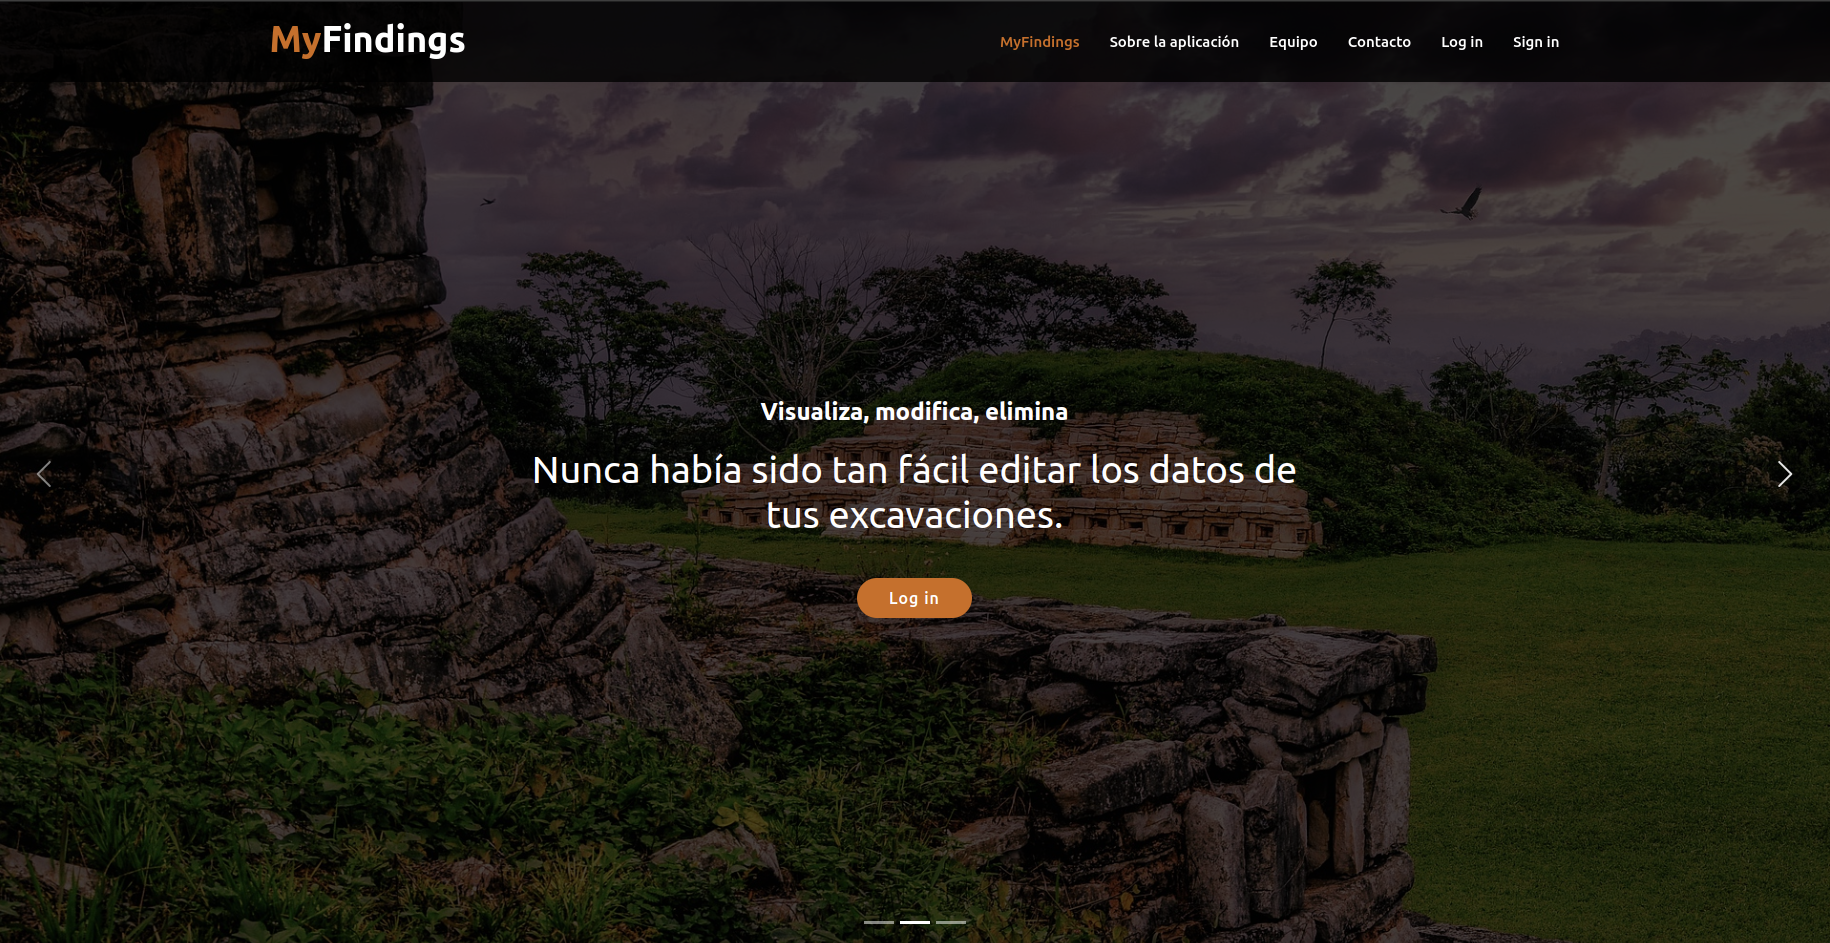
\includegraphics[scale=0.17]{imagenes/home.png}
            \caption{Home de la página}
            \label{fig:home}
        \end{figure}

    \subsection{Listados}
    Esta parte de la vista corresponderá a distintas vistas que servirán para listar en forma
    de \textbf{tablas} las distintas excavaciones, estancias, hechos, unidades estratigráficas
    (sedimentarias y construidas), fotografías, materiales (sedimentarios y construidos) e
    inclusiones.\\

    Principalmente corresponderá a tablas donde además de la información propia
    de los registros se muestren las posibilidades de editar y eliminar dichos registros
    residentes en la base de datos, que como dijimos en la sección de análisis, va a ser
    PostgreSQL. Esta parte de la implementación se explicará en secciones posteriores.

    \subsection{Añadir}
    Esta sección de la página web corresponderá a las distintas vistas (formularios) que
    servirán para añadir los distintos componentes relacionados con las excavaciones:
    excavaciones, estancias, hechos, unidades estratigráficas (sedimentarias y construidas),
    fotografías, materiales (sedimentarios y construidos) e inclusiones.\\

    Cada uno de estos formularios pedirá al usuario los datos completos de cada elemento del
    que se trate, por supuesto, con la posibilidad de dejar algún campo en blanco, aunque
    no sería lo más normal ya que en el servidor web la idea es rellenar de forma completa
    la información que se recopile en el registro de campo con la aplicación android, además
    de añadir otra información.

    \subsection{Sobre la aplicación}
    En esta página de la web se hace alusión brevemente a cuál es la principal motivación
    de crear este proyecto y cuales son las principales características que posee la
    aplicación: \textit{sincronización en tiempo real con la aplicación android, fácil
    adición, edición y eliminación de información de los distintos elementos, generación
    de informes a partir de la información de la base de datos, etc}.\\

    Dicha página quedaría de la siguiente forma:
        
        \begin{figure}[H]
            \centering
            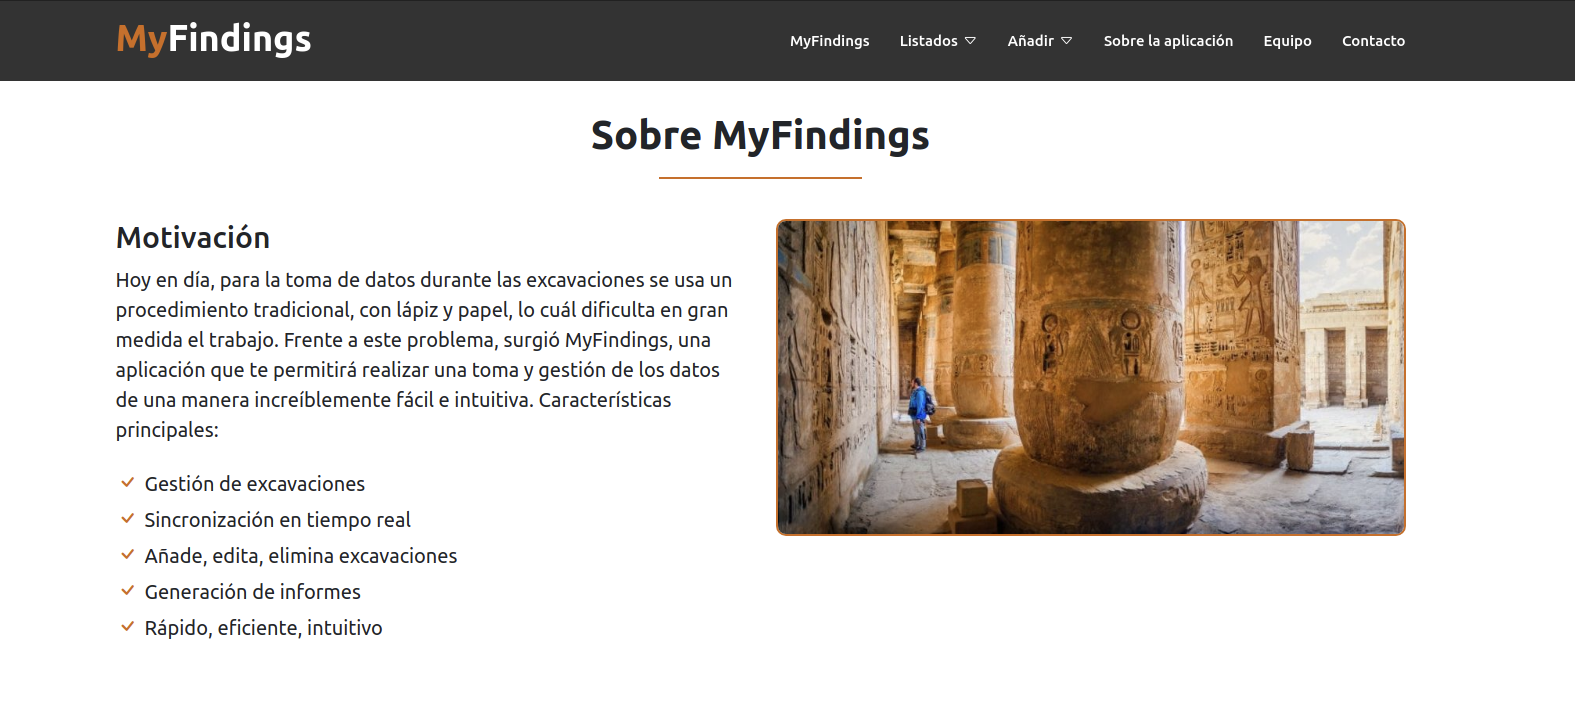
\includegraphics[scale=0.20]{imagenes/about.png}
            \caption{Sobre la aplicación}
            \label{fig:about}
        \end{figure}

    Como puede observarse, esta página está formada por dos rows, el primero, que se
    corresponde con el \textbf{headline} (común en muchas páginas) y el segundo, que está
    dividido en dos partes que usan 6 columnas de Bootstrap cada una, conteniendo la
    \textbf{motivación} y la \textbf{imagen}.

    \subsection{Equipo}
    Esta página contiene información sobre los componentes que hemos hecho posible este
    proyecto, en este caso, \textit{Joaquín García Venegas} y yo, \textit{Joaquín
    Alejandro España Sánchez}\\
    
    Por supuesto, ambos hacemos funciones totalmente distintas, por un lado la aplicación
    android y por otro la aplicación web, sobre lo que nos centraremos en este proyecto.
    Ambos componentes son diferentes, pero en su conjunto forman \textbf{MyFindings},
    un proyecto completamente funcional. La página quedaría tal que así:

        \begin{figure}[H]
            \centering
            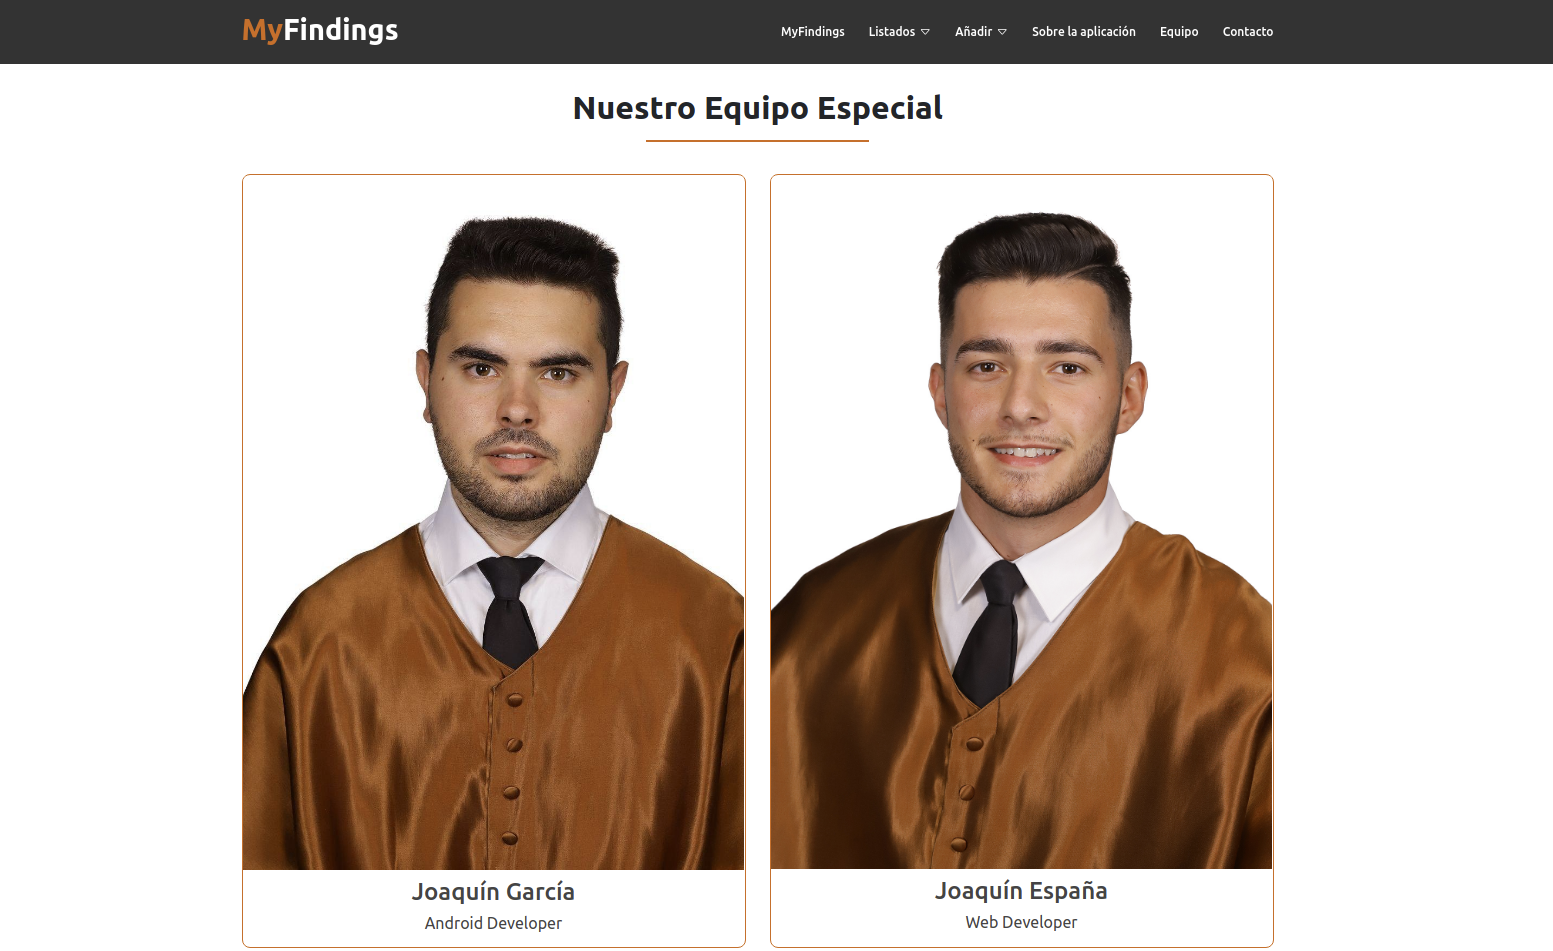
\includegraphics[scale=0.20]{imagenes/team.png}
            \caption{Equipo de MyFindings}
            \label{fig:team}
        \end{figure}

    En este caso se ha utilizado una estructura de página muy parecida a la anterior, utilizando
    dos rows, el primero para el \textbf{headline} y el segundo para los \textbf{miembros} del
    proyecto. Cabe mencionar el uso de la clase \textbf{border-box} en numerosas ocasiones en 
    el código, éste incorpora un border naranja al componente que lo posea.

    \subsection{Contacto}
    Finalmente, tenemos la página de contacto de la aplicación web, en ella podemos
    encontrar datos como el correo electrónico del desarrollador y su página de
    \href{https://github.com/alexespana/}{Github} o un mapa del lugar de residencia del
    programador, en este caso Granada.\\

        \begin{figure}[H]
            \centering
            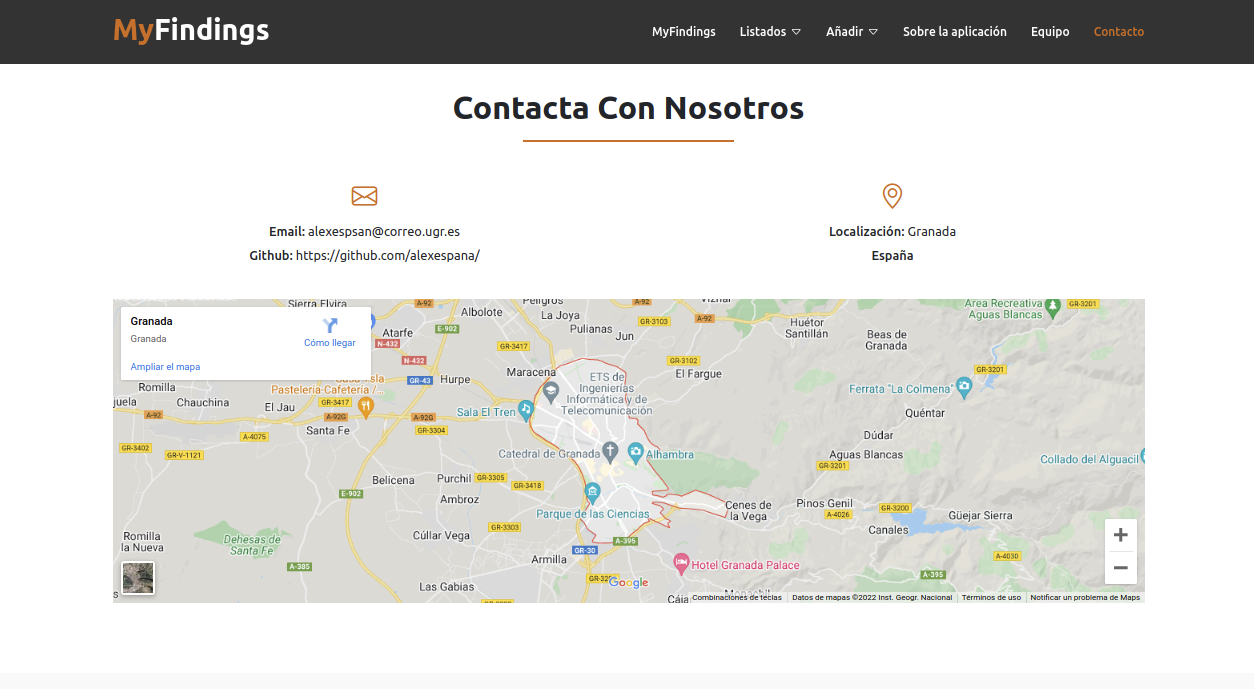
\includegraphics[scale=0.25]{imagenes/contact.png}
            \caption{Contacto de MyFindings}
            \label{fig:contact}
        \end{figure}

    Para realizar esta página se ha hecho uso de tres filas, la primera de ellas
    está destinada al \textbf{headline}, que como hemos visto, es común en otras páginas, 
    por lo que usan la misma clase de estilo CSS. La segunda a su vez está dividida en 
    dos partes utilizando cada una 6 columnas y finalmente la tercera fila ha sido
    destinada para el \textbf{iframe} de google maps cuyo código html ha sido extraído
    directamente de la aplicación web y puesto sobre el código.

\section{Database creation}
Este milestone es uno de los más importantes del proyecto ya que tiene como principal objetivo
la definición de la base de datos que se utilizará, que posteriormente nos permitirá hacer las
consultas apropiadas según las necesidades que busca el cliente, en este caso los arqueólogos.\\

No prestarle atención a este hito sería un grave error, ya que si se realiza un mal diseño
de la BD puede conducir a las siguientes consecuencias en el desarrollo de software:

    \begin{itemize}
        \item El proyecto podría \textbf{fallar} al no soportar los requerimientos de la
        aplicación.
        \item Si hay un diseño muy complejo, el costo de desarrollo se verá
        \textbf{incrementado} ya que habrá que implementar más código para solucionar las
        distintas dificultades de la DB.
        \item Una base de datos compleja puede tener \textbf{gran cantidad de tablas} que 
        provocan código innecesario y complejo de entender.
        \item Posibles relaciones erróneas entre los datos que pueden llegar a provocar
        \textbf{fallos en la actualización} de los mismos y que finalmente sea necesario realizar
        actualizaciones manuales.
    \end{itemize}

En este caso, necesitamos utilizar una \textbf{base de datos relacional} ya que gran número
de tablas están relacionadas entre sí, existiendo claves externas e incluso claves
candidatas que se forman a partir de claves primarias y atributos discriminadores de
relaciones. Todo esto, se verá en la sección siguiente.

    \subsection{Modelo E/R}
    El modelo E/R es la técnica de modelado de datos más extendida para el diseño
    conceptual ya que posee una gran capacidad expresiva (a simple vista se pueden
    distinguir las distintas entidades con sus atributos y relaciones), es rigurosa, simple
    y fácil de emplear. Nos permite especificar las necesidades de información de nuestro
    proyecto permitiéndonos hacer un diseño \textbf{\textit{apropiado}},
    \textbf{\textit{de calidad}} y \textbf{\textit{fácil de transmitir}}.\\

    Para realizar dicho diseño, se ha hecho conjuntamente con \textit{Joaquín García 
    Venegas}, ya que para la aplicación android también será necesario tener el diseño de la
    BD. Este modelo deberá:

        \begin{enumerate}
            \item Reflejar fielmente las necesidades de información del proyecto. Ésto permite
            partir de una base para el desarrollo del sistema.
            \item Ofrecer un diseño independiente a la forma en que los datos serán
            posteriormente almacenados y sus formas de acceso, permitiendo tomar decisiones
            objetivas sobre la implementación más idónea.
        \end{enumerate}

    Teniendo todo esto en cuenta, el modelo E/R resultante para nuestro proyecto es el
    siguiente:

        \begin{figure}[H]
            \centering
            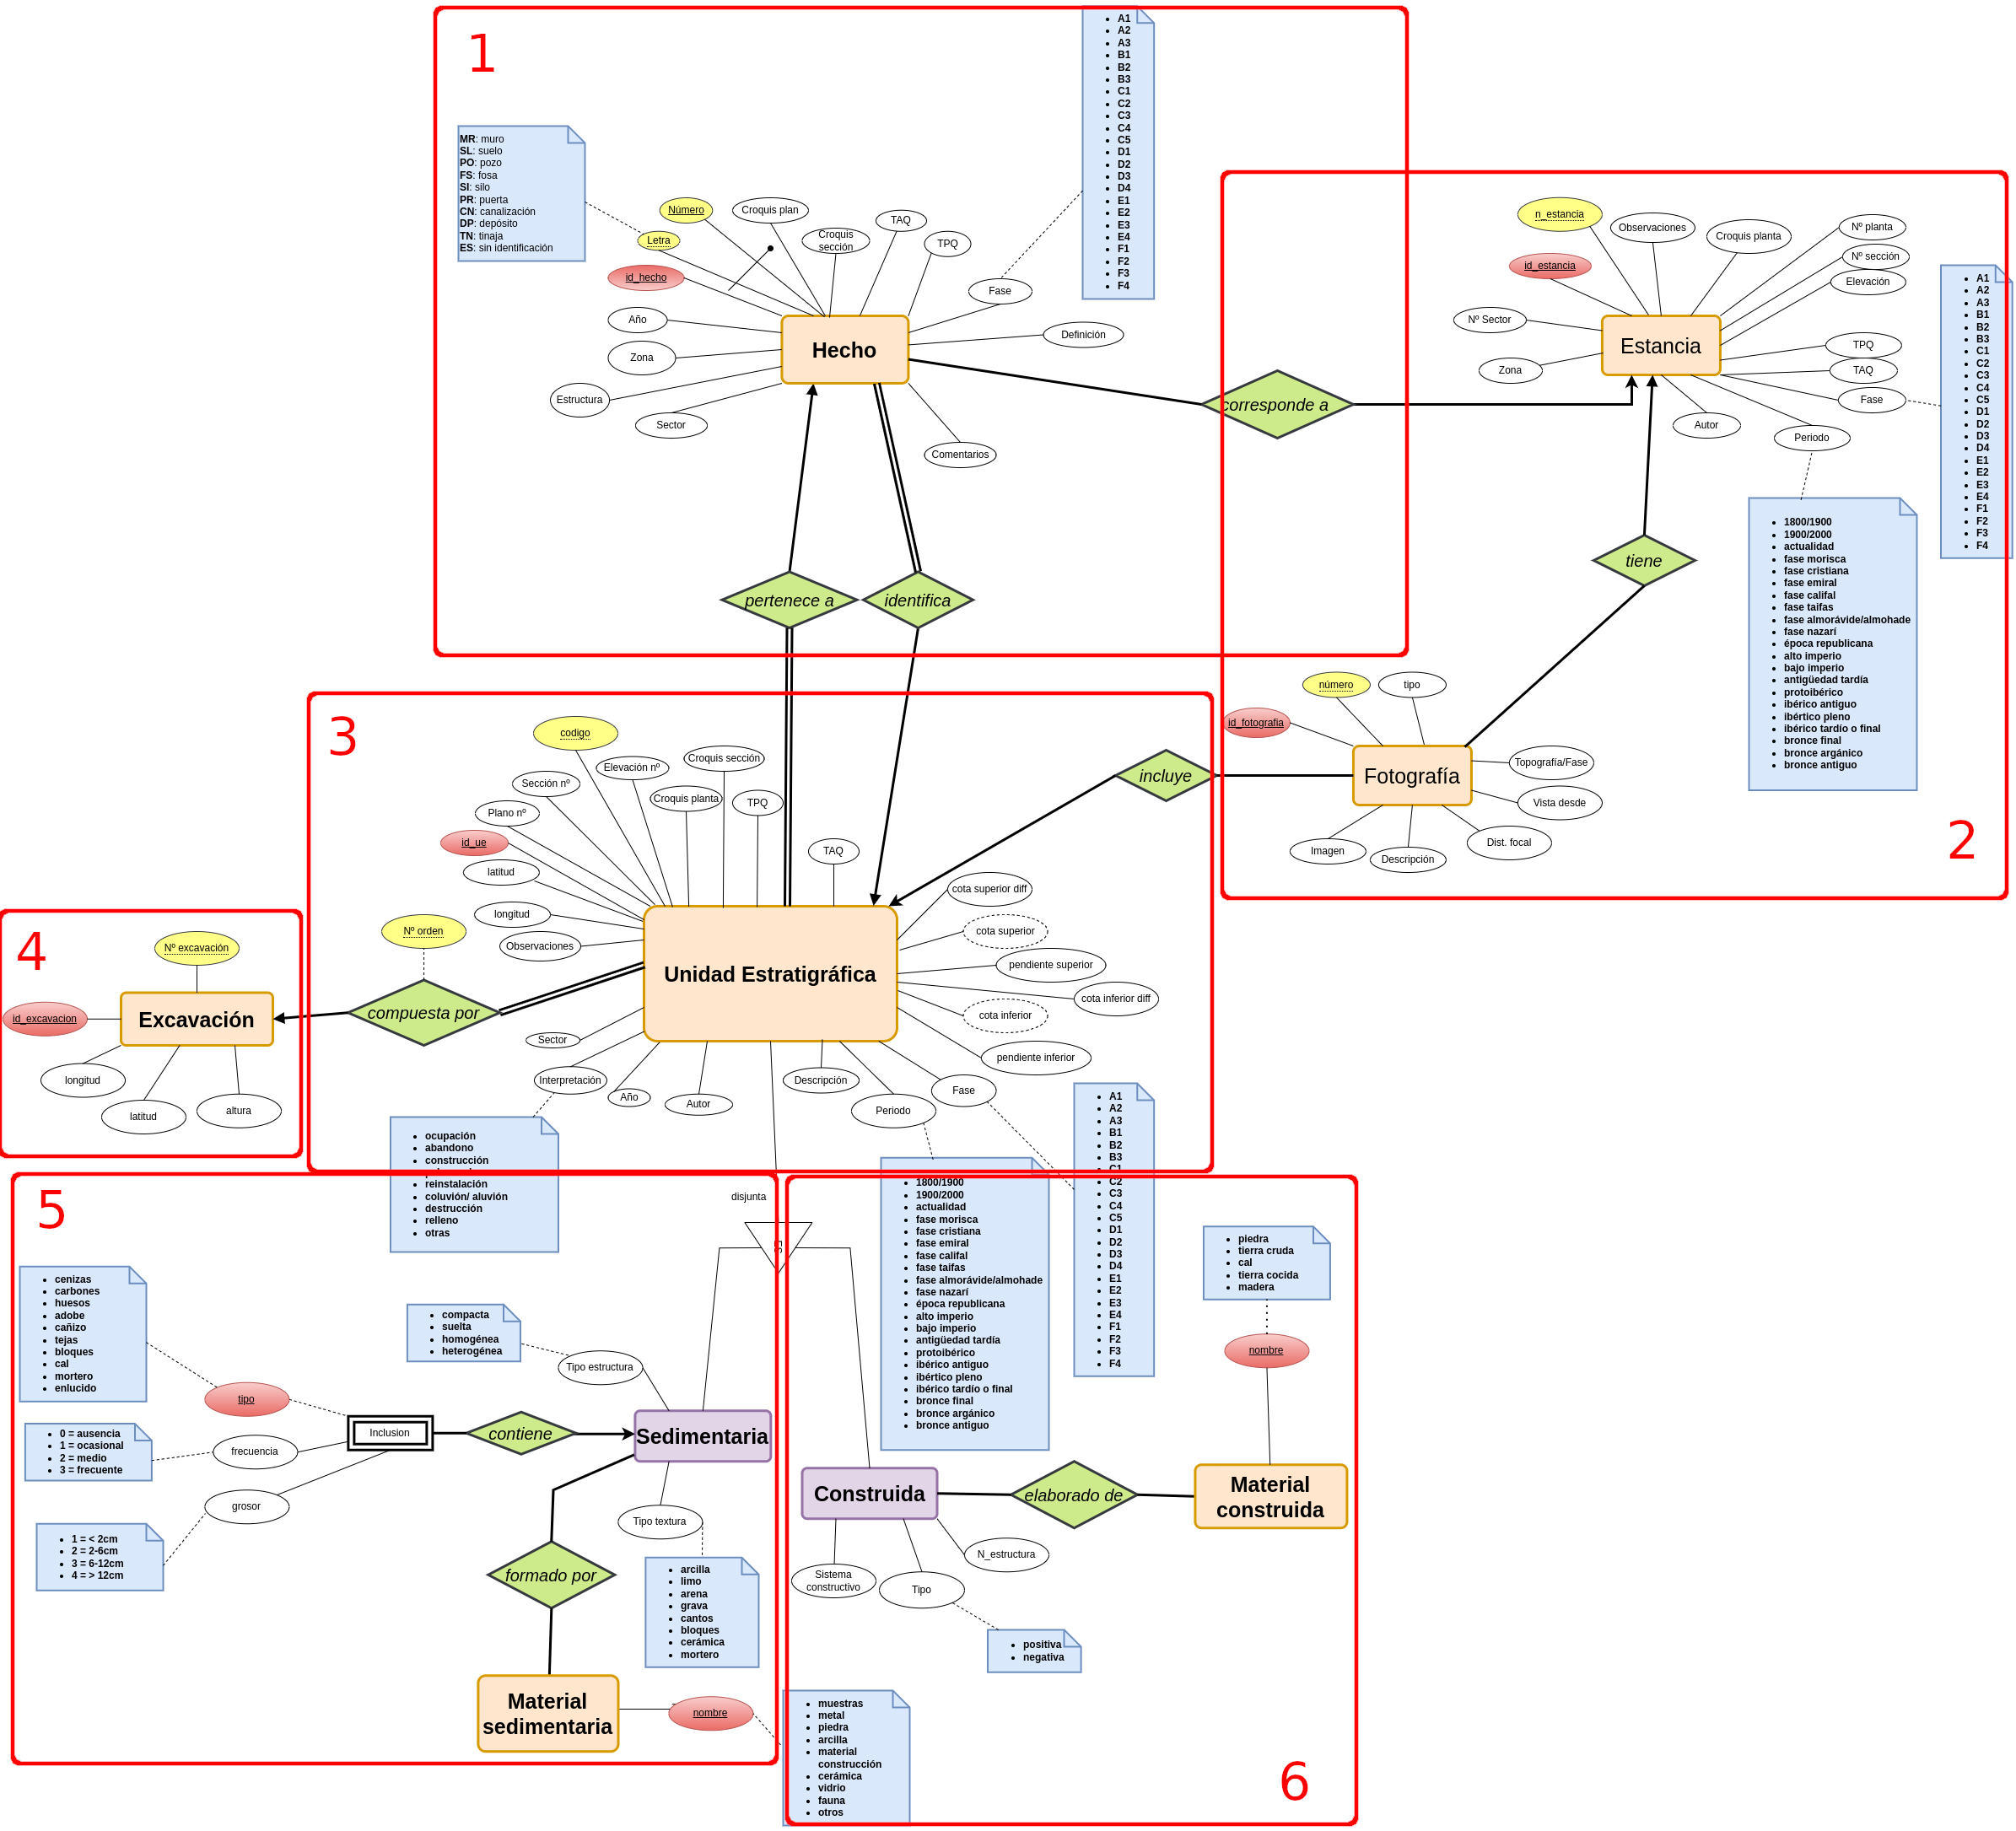
\includegraphics[scale=0.10]{imagenes/E-RModel.png}
            \caption{Modelo Entidad/Relación}
            \label{fig:e-rmodel}
        \end{figure}

    Vamos a comenzar justificando las elecciones más importantes que se han ido tomando
    sobre el modelo, para ello seguiré el siguiente orden: \textbf{entidades fuertes},
    \textbf{herencia}, \textbf{entidades débiles} y \textbf{relaciones}.\\

    \subsubsection{Entidades fuertes}
    Como podemos observar, hay siete entidades fuertes, entre las que podemos destacar,
    además de los atributos necesarios que no son claves primarias o candidatas, lo siguiente:

    \begin{enumerate}
        \item \textbf{Excavación}: ésta tendrá un identificador interno en la base de
        datos que actuará como primary key, que será un valor numérico, y además una clave
        candidata que será el \textbf{número de excavación}, un entero de tres dígitos
        (p.ej: 001, 043, 132, etc). Esta clave candidata será la visible al usuario, pudiendo
        introducir el número de excavación deseado.

        \item \textbf{Unidad Estratigráfica}: al igual que la anterior, tendremos un
        identificador interno que será la primary key, y además, una clave candidata que
        será el \textbf{código} de la unidad estratigráfica, que servirá para que el usuario
        pueda identificar dicha unidad. Dicho código debe estar formado por el
        \textbf{número de excavación} al que pertenece la unidad más el \textbf{número de orden}
        de la unidad en la excavación. Por ejemplo, si la unidad pertenece a la excavación
        \textbf{001} y es la unidad número 32 encontrada en la excavación (\textbf{032}), el
        código que identificaría a la unidad sería el \textbf{001032}.

        \item \textbf{Hecho}: la forma que tiene el usuario de identificar a cada hecho es algo
        más compleja. Al igual que las dos entidades anteriores, también se tendrá un
        identificador interno que actuará de primary key, y además, se tendrá una clave
        candidata compuesta, que estará formada por la \textbf{letra} (tipo de hecho) y un
        \textbf{número}. Para poder darle un valor coherente a este número, se elige una
        unidad estratigráfica perteneciente al hecho y el código de dicha unidad será el
        número(\textbf{parte de la clave candidata}) de dicho hecho. Por ejemplo, si tenemos
        la unidad estratigráfica con código \textbf{001032} y dicha unidad es la que sirve
        para identificar al hecho de tipo muro (\textbf{MR}) la clave candidata del hecho
        sería \textbf{MR001032}.

        \item \textbf{Estancia}: en este caso, al igual que las entidades anteriores,
        tendremos un identificador interno como primary key que solo se conocerá internamente
        en el sistema, y además, tendremos un \textbf{número de estancia}, que será la clave
        candidata de la entidad, visible y reconocible para los usuarios de la aplicación. Al
        comienzo del diseño pensábamos que el número de estancia se formaba a partir del número
        de sector y el número de zona, como está reflejado en el anexo \ref{subsec: doubts},
        pero finalmente éste esta formado por las letras ES seguidas de tres dígitos. Por ejemplo
        un posible identificador de estancia podría ser \textbf{ES001}.

        \item \textbf{Fotografía}: poseeremos un primary key interno para la entidad y una
        clave candidata que será el \textbf{número} de la fotografía. Las fotografías están
        relacionadas tanto con las unidades estratigráficas como con las estancias, y es que 
        ambas pueden tener fotografías concretas.
        
        \item \textbf{Material construido}: esta entidad surge porque una unidad estratigráfica
        construida puede estar construida con \textbf{varios tipos de materiales} construidos,
        de ahí el hecho de que no se pueda poner simplemente un atributo que sea material en
        la unidad construida y se tenga que añadir una nueva entidad.

        Al comienzo podría pensarse que el material es una entidad débil de la unidad
        construida, pero esto traería problemas ya que para identificar a un material sería
        necesario el identificador de la unidad estratigráfica y el atributo discriminador de
        la entidad débil. Esto carecería de sentido ya que podría haber dos UE's construidas
        con el mismo material, pero cada uno se identificaría de una forma distinta, a pesar
        de ser el mismo material. Por esta razón se consideró como una entidad fuerte, a la
        que muchas unidades estratigráficas construidas pueden estar asociadas. Tiendo esto
        en cuenta, esta vez no tendremos un primary key interno, sino que el \textbf{nombre}
        del material será la primary key. Por ejemplo: el material \textbf{Piedra} pudiese
        formar parte de 50 unidades construidas, siendo únicamente necesario el 
        \textbf{nombre} del material para identificar a uno.
        
        \item \textbf{Material sedimentario}: esta entidad, al igual que la anterior, surge
        porque una unidad estratigráfica sedimentaria puede estar construida con 
        \textbf{varios tipos de materiales} sedimentarios, de ahí el hecho de que no se pueda
        poner simplemente un atributo que sea material en la unidad sedimentaria y se tenga que
        añadir una nueva entidad.

        En este caso también podríamos pensar que el material es una entidad débil de la unidad
        sedimentaria, pero esto también traería problemas ya que para identificar a un material
        sería necesario el identificador de la unidad sedimentaria y el atributo discriminador
        de la entidad débil, que en este caso sería el \textbf{nombre}. Como hemos mencionado
        anteriormente, no tiene sentido ya que podría haber dos UE's sedimentarias hechas
        con el mismo material, pero cada uno se identificaría de una forma distinta, a pesar
        de ser el mismo material. Por esta razón se consideró como una entidad fuerte, a la
        que muchas unidades estratigráficas sedimentarias pueden estar asociadas. Igual que el
        anterior, la primary key sería el \textbf{nombre} del material. Por ejemplo: el
        material \textbf{Metal} pudiese formar parte de 10 unidades sedimentarias, siendo
        únicamente necesario el \textbf{nombre} del material para identificar a uno. 
    \end{enumerate}

    \subsubsection{Herencia}
    Como podemos comprobar en el modelo E/R, existen claramente dos entidades que heredan de
    la entidad fuerte Unidad Estratigráfica, la \textbf{Sedimentaria} y la \textbf{Construida}.
    Ambas heredarán todos los atributos de la entidad padre y además añadirán sus propios
    atributos. En las fichas de registro de campo completo \ref{sec:registrationforms} puede
    verse en la UE construida como existe un apartado material, sin embargo, en la sedimentaria
    no existe una sección como tal, la pregunta sería: \textbf{¿por qué las UE sedimentarias
    tienen un material distinto entonces?} Tras numerosas entrevistas con el arqueólogo al
    final se dedujo que los materiales de la primera hoja de \ref{sec:registrationforms}
    correspondian a materiales que sólo las UE's sedimentarias podían tener, por esta razón
    se incorporaron.

    \subsubsection{Entidades débiles}
    La única entidad débil del modelo E/R es la \textbf{Inclusión}. Dicha entidad surge porque
    una inclusión posee distintos atributos como la \textbf{frecuencia}, el \textbf{grosor} y
    el \textbf{tipo}, por lo que habría que modelarlos como una entidad que recogiese todos
    estos datos, además de que una unidad sedimentaria podría tener varias de ellas. En este
    caso, sí tiene sentido reflejarla como una \textbf{entidad débil} ya que las inclusiones
    son propias de cada UE y no se comparten con otras unidades sedimentarias.\\

    Por lo tanto, estaría identificada por el \textbf{identificador} de la unidad estratigráfica
    sedimentaria y el atributo discriminador de la entidad débil que en este caso es el
    \textbf{tipo} (que puede ser cenizas, carbones, huesos, adobe, etc).

    \subsubsection{Relaciones}
    Finalizando con las relaciones, voy a enumerar las distintas relaciones identificando las
    entidades implicadas:

        \begin{enumerate}
            \item \textbf{Compuesta por (Excavación-UE)}: relación uno a muchos (1:M). En la
            relación se guarda el número de orden de la unidad estratigráfica.
            \item \textbf{Pertenece a (UE-Hecho)}: relación muchos a uno (M:1).
            \item \textbf{Identifica (UE-Hecho)}: relación uno a muchos (1:M).
            \item \textbf{Corresponde a (Hecho-Estancia)}: relación muchos a 1 (M:1).
            \item \textbf{Tiene (Estancia-Fotografía)}: relación uno a muchos (1:M).
            \item \textbf{Incluye (Fotografía-UE)}: relación muchos a uno (M:1).
            \item \textbf{Contiene (Sedimentaria-Inclusión)}: relación 1 a muchos (1:M).
            \item \textbf{Formado por (Sedimentaria-Material sedimentaria)}: relación muchos a
            muchos (M:N).
            \item \textbf{Elaborado de (Construida-Material construida)}: relación muchos a
            muchos (M:N).
        \end{enumerate}

    \subsection{Django ORM}
    Ahora vamos a hablar un poco sobre la implementación \textbf{en el código}, en la forma
    de representar el modelo E/R en nuestra aplicación \textbf{Django}.\\

    \subsubsection{¿Qué es un ORM?}
    Antes de nada, vamos a explicar qué es un \textbf{ORM (Object Relational Mapping)}, ya
    que será un concepto clave para entender lo posteriormente explicado. Un ORM es un modelo
    de programación que nos permite mapear las estructuras de una base de datos relacional
    sobre unas estructuras lógicas en el código (por ejemplo objetos), es decir, nos permite
    convertir los objetos de nuestra aplicación en un formato adecuado (SQL) para ser
    almacenado en la base de datos. Como todo en la vida, esto tiene unas ventajas y unas
    desventajas, comencemos por las ventajas:

        \begin{enumerate}
            \item Hacen que el proceso de desarrollo sea más rápido.
            \item No se necesita tener \textbf{conocimiento de SQL } para usar el ORM. Esto
            hace que la complejidad del DML se reduciese, evitando tener que hacer joins,
            multi-inserciones, sub-selecciones, etc.
            \item El ORM asegura la consulta para cualquier tipo de ataque.
        \end{enumerate}

    A pesar de tener cosas muy buenas, el ORM también tiene algunos aspectos que podrían
    considerarse pequeñas desventajas:

        \begin{enumerate}
            \item Los ORMS generan una consulta y la pasan a la base de datos. En ocasiones
            estas consultas devuelven una matriz con un formato complejo con
            \textbf{colecciones}(objetos) que tienen información no relevante para nosotros
            \item Cuando la lógica de negocio de la aplicación se vuelve compleja, a veces
            no se puede representar mediante un ORM, aunque sí pueda ser manejable a nivel
            de consulta
        \end{enumerate}

    Dicho todo esto, podemos comenzar a hablar sobre el ORM que utilizaremos para la
    aplicación web, el \textbf{ORM de Django}. Éste nos permite diseñar nuestras tablas de 
    base de datos sin necesidad de escribir ninguna sentencia SQL, en este caso, en
    \textbf{PostgreSQL}. Un modelo es la fuente de información única y definitiva para los
    datos, éste contendrá los campos y funcionalidades(comportamiento) correspondientes a
    la naturaleza de los datos que almacena. Normalmente, cada modelo se asigna a una sola
    tabla de base de datos, y cada uno de ellos:

        \begin{itemize}
            \item Es una clase de python que hereda de la clase \textbf{django.db.models.Model}.
            \item Cada atributo de la clase representa un campo (columna) de la base de datos.
            \item Al corresponderse cada entidad a una clase, Django proporciona automáticamente
            una \textbf{API de abstracción de bases de datos} que nos permite realizar las
            operaciones de \textbf{CRUD} básicas: crear, recuperar, actualizar y eliminar
            objetos.
        \end{itemize}

    Cada modelo visible para el usuario tiene una función \textbf{\textit{str}} que se
    corresponde con la identificación del objeto al mostrarlo al usuario. Digamos que se
    trata de un método especial que devuelve una representación en forma de \textbf{string} de
    cualquier objeto y que Python y Django utilizarán cada vez que una instancia de un 
    modelo necesite ser mostrada como una cadena, como puede ser en el caso de la consola
    interactiva, en la vista de administrador, en un display de una tabla, etc.\\

    Pongamos un ejemplo, si la unidad estratigráfica posee un \textbf{ForeignKey} que es
    la \textbf{excavación} a la que pertenece, dicha instancia de excavación se mostraría
    para el usuario como el \textbf{número de excavación}, ya que en el modelo de la
    excavación existirá un método str que devolvería el \textbf{n\_excavacion},
    quedando el modelo de la siguiente forma:

    % DESCOMENTAR
    \begin{minted}[mathescape, linenos,numbersep=5pt,bgcolor=lightgray,gobble=2,
                   frame=lines,fontsize=\footnotesize,framesep=2mm]{python}
    class Excavacion(models.Model):
        n_excavacion = models.PositiveIntegerField(unique=True, 
                        verbose_name='Número de excavación')
        latitud = models.FloatField()
        longitud = models.FloatField()
        altura = models.PositiveSmallIntegerField()

        def __str__(self):
            return str(self.n_excavacion)
    \end{minted}

    Si nos fijamos, vemos que es necesario que esta función devuelva un string, por esta
    razón se usa la función str en el return. Además, Django nos proporciona \textbf{gran
    variedad de tipos posibles} para los campos de los modelos, por lo que nos podemos
    ahorrar hacer algunas comprobaciones en los formularios de recogida de datos, aunque
    algunas serán necesariamente obligatorias. Aquellos campos que necesiten ser positivos
    utilizarán campos de tipo \textbf{PositiveSmallIntegerField}, que nos permite introducir
    enteros desde el 0 hasta el 32767, cantidades suficientes para el contexto de nuestro
    proyecto.\\

    Lo siguiente va a ser explicar cómo representar en los modelos las \textbf{primary keys},
    \textbf{candidate keys} y \textbf{relationships}.\\
    
    \subsubsection{Primary keys}
    En los atributos de los modelos, en los tipos de campo, existe un parámetro llamado
    \textbf{primary\underline{ }key}, si se indica a True, entonces dicho campo será la clave
    primaria del modelo, pero si no se indica el primary key en ningún campo del modelo,
    entonces django automáticamente añadirá un campo \textbf{id} para guardar la clave primaria.
    Dicho atributo será un campo de tipo \textbf{models.BigAutoField}, que nos permite números
    desde el 1 hasta el 9223372036854775807, por lo que no habrá ningún tipo de problema con
    la generación de los id's. Por supuesto, si en algún campo se declara \textbf{explícitamente}
    la clave primaria, django no generará el campo id y el campo que hayamos elegido pasará a
    ser clave primaria. En nuestro modelo E/R, las claves primarias que se generarán
    automáticamente por django en los modelos serán las de \textbf{Excavacion, UE, Hecho,
    Estancia y Fotografia}. 
    
    \subsubsection{Candidate keys}
    Para las \textbf{claves candidatas simples} únicamente hay que indicar en el campo
    correspondiente al argumento \textbf{unique} a True. Por ejemplo, en el modelo
    \textbf{Excavación} mostrado anteriormente el campo del número de excavación es
    candidate key:
    
    % DESCOMENTAR
    \begin{minted}[mathescape, linenos,numbersep=5pt,bgcolor=lightgray,gobble=2,
                   frame=lines,fontsize=\footnotesize,framesep=2mm]{python}
    class Excavacion(models.Model):
        n_excavacion = models.PositiveIntegerField(unique=True, 
                        verbose_name='Número de excavación')
        .
        .
    \end{minted}

    ¿Cómo se representaría una clave candidata compuesta? En Django, esto se puede hacer de
    dos formas posibles:

    \begin{enumerate}
        \item Mediante la opción \textbf{unique\underline{ }together}, que incluye la lista
        de campos que formarán la clave candidata, y que por lo tanto conjuntamente serán
        únicos. Vamos a hacer el ejemplo con el modelo Hecho, ya que es el único que tiene
        una clave candidata compuesta:
        
    % DESCOMENTAR
    \begin{minted}[linenos,numbersep=5pt,bgcolor=lightgray,gobble=2,
        frame=lines,fontsize=\footnotesize,framesep=2mm]{python}
    class Excavacion(models.Model):
        letra = models.CharField(max_length=2, choices=LETRA_CHOICES)
        numero = models.CharField(max_length=6)    
        .
        .
        class Meta:
            unique_together = ('letra', 'numero',)
    \end{minted}

        \item La forma anterior, sin embargo, no es del todo aconsejable por django ya
        que sugiere utilizar \textbf{UniqueConstraint} con la opción \textbf{constraint},
        ya que la opción de \verb|unique_together| ofrece menor funcionalidad y puede
        estar deprecated en un futuro. Con esta nueva forma, la clase de metadatos
        del modelo quedaría así:
        
    % DESCOMENTAR
    \begin{minted}[linenos,numbersep=5pt,bgcolor=lightgray,gobble=2,
        frame=lines,fontsize=\footnotesize,framesep=2mm]{python}
    class Excavacion(models.Model):
        letra = models.CharField(max_length=2, choices=LETRA_CHOICES)
        numero = models.CharField(max_length=6)    
        .
        .
        class Meta:
            constraints = [
                models.UniqueConstraint(fields=['letra', 'numero'], 
                                        name='fact_constraint')                                                  
            ]
    \end{minted}

    Dicha restricción tendrá el nombre de \textbf{fact\underline{ }constraint}.
    \end{enumerate}

    \subsubsection{Relationships}
    Django soporta las mismas tres relaciones que existen en una base de datos relacional:
    uno a uno, uno a muchos, y muchos a muchos. Para representarlas, usa tres tipos de campos
    para los modelos, que son:

        \begin{itemize}
            \item \textbf{OneToOneField}: en uno de los modelos implicados, recibe como
            argumentos básicos el nombre del modelo con el que está asociado y el argumento
            del borrado en cascada (\textbf{on\underline{ }delete}).
            \item \textbf{ForeignKey}: en el modelo de la parte \textbf{muchos}, irá un campo
            con el nombre del modelo asociado en minúscula y de tipo ForeignKey, recibiendo
            como parámetros el nombre del modelo asociado (parte del uno) y el argumento del
            borrado en cascada.
            \item \textbf{ManyToManyField}: este tipo de relaciones son algo más complejas. Al
            ser una relación M:N podemos pensar que en cada uno de los modelos irá un campo
            ManyToManyField, pero esto no es así. En el modelo donde tenga más lógica que vaya
            el campo muchos a muchos irá un campo con el nombre del otro modelo en plural(por
            \textbf{convención}) con el dato de tipo ManyToManyField, que recibe como parámetro
            únicamente el nombre del modelo con el que se relaciona.

            Por ejemplo, tengamos los modelos Pizza y Topping, ¿qué se entiende mejor?
            \textbf{¿que una pizza pueda tener muchos toppings?}, \textbf{¿o que un
            topping pueda estar en muchas pizzas?} La primera de las opciones es más
            intuitiva y por tanto el modelo Pizza tendría un campo toppings de tipo
            ManyToManyField.
        \end{itemize}

    Explicadas las formas de representar las relaciones en Django, voy a mencionar las
    relaciones que se dan en nuestro modelo:

        \begin{enumerate}
            \item El \textbf{Hecho} tiene una clave externa referenciando a la estancia a la
            que está asociado.
            \item La \textbf{UE}(unidad estratigráfica) tiene dos claves externas, una
            referenciando a la excavación con la que está asociada y otra referenciando al
            hecho al que pertenece.
            \item La \textbf{Fotografia} tiene también dos claves externas, una referenciando
            a la unidad estratigráfica asociada y otra referenciando a la estancia.
            \item La \textbf{Inclusion} tiene una clave externa referenciando la unidad
            estratigráfica sedimentaria a la que pertenece.
            \item La \textbf{UESedimentaria} tiene un campo ManyToManyField referenciando a
            los materiales sedimentarios (\textbf{MaterialSedimentaria}) por los que está
            formada.
            \item La \textbf{UEConstruida} tiene un campo ManyToManyField referenciando a
            los materiales construidos (\textbf{MaterialConstruida}) por los que está
            formada.
        \end{enumerate}

    Esta sería una visión global de la implementación utilizando el ORM que nos ofrece Django.
